%-------------------------------------------------------%
\section{概要} \label{sec:tutrial_real_intro}
%-------------------------------------------------------%
このチュートリアルでは、現実大気の基本的な実験方法を習得する。
現実大気実験は、次の流れ(図\ref{fig:howto}) に従って実行する。
\begin{enumerate}
\item  入力データの準備 (基本各自で準備。チュートリアルでは \verb|tools/| で行う。)
\item  \texttt{pp}      : 地形・土地利用データの作成
\item  \texttt{init}    : 初期値・境界値データの作成
\item  \texttt{run}     : 初期条件を作るディレクトリ
\item  \texttt{net2g}   : 出力データの\netcdf から\grads 形式への変換(オプション) 
\end{enumerate}

\begin{figure}[b]
\begin{center}
  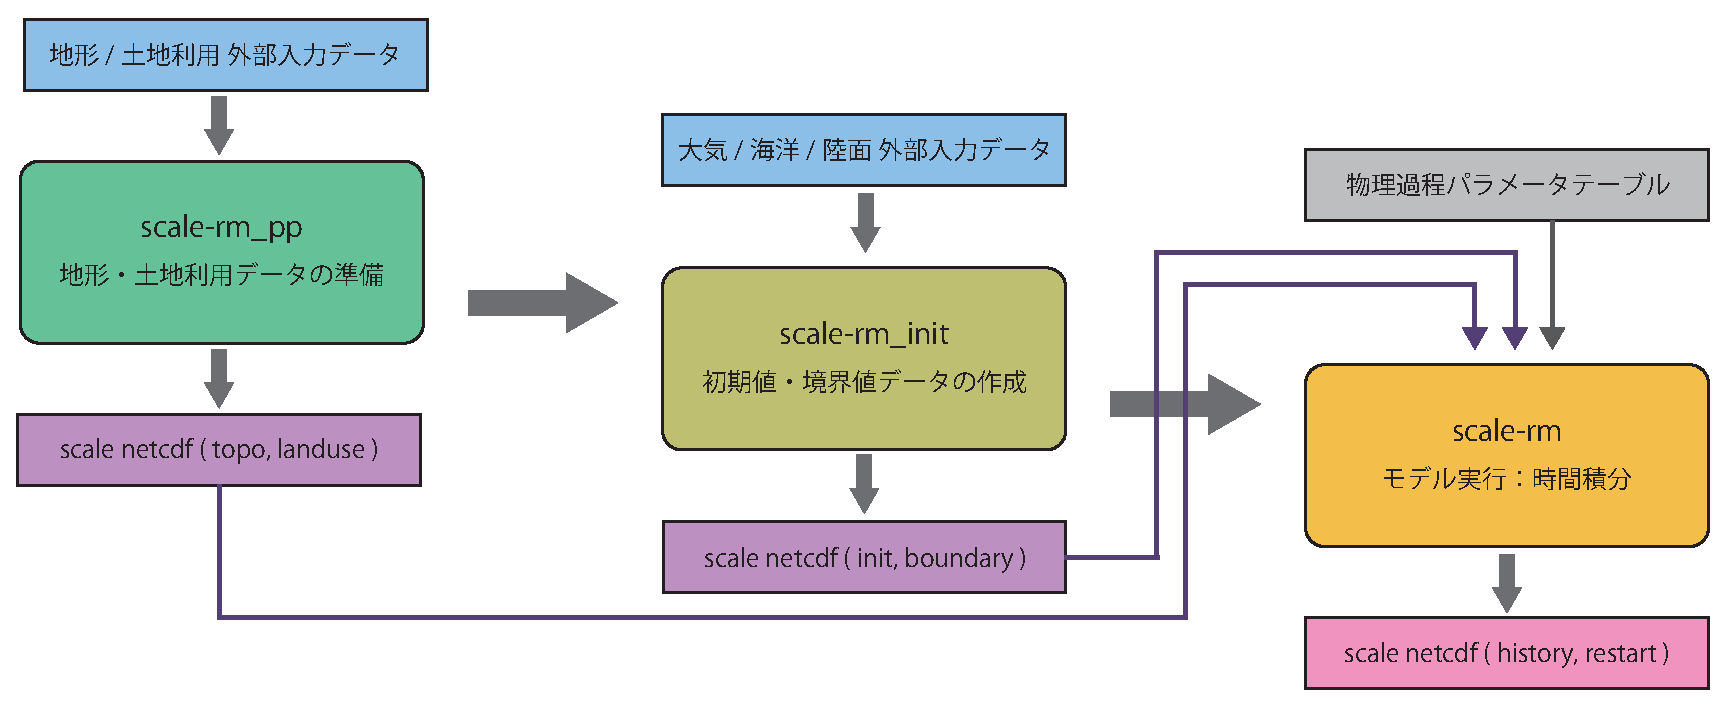
\includegraphics[width=0.9\hsize]{./figure/real_procedure.eps}\\
  \caption{\scalerm モデルの実行過程}
  \label{fig:howto}
\end{center}
\end{figure}


チュートリアルの現実大気実験の計算領域(ドメイン)の設定は表\ref{tab:grids}のようになっている。
図 \ref{fig:tutrial_real_domain}に対象領域を示す。
このチュートリアルは、\scalerm の使い方を学ぶことが目的であり、
短い時間で実行可能な設定にしている。
領域モデルの実験設定として必ずしも適切な設定を選択しているとは限らないので
ご留意頂きたい
(例えば、20kmの水平解像度で積雲パラメタリゼーションなし)。
本章のチュートリアルを比較的短時間で実行するには、下記の条件を満たす計算機環境が推奨される。
\begin{itemize}
\item CPU: 2コア/4スレッド以上の演算コアを持つCPU(4コア以上を推奨)
\item Memory容量: 4GB以上をプログラムに割当可能(8GB以上を搭載した計算機を推奨)
\item HDD空き容量: 7GB以上の空き容量
\end{itemize}


\begin{table}[h]
\begin{center}
  \caption{実験設定の概略}
  \label{tab:grids}
  \begin{tabularx}{150mm}{|l|X|} \hline
    \rowcolor[gray]{0.9} 項目 & 設定 \\ \hline
    MPIプロセス分割 (東西 x 南北) & 2 x 2 (合計4プロセス) \\ \hline
    水平格子数 (東西 x 南北) & 90格子点 x 90格子点 \\ \hline
    鉛直層数                 & 36層                  \\ \hline
    水平格子間隔             & dx = dy = 20km       \\ \hline
    積分期間 & 2007年7月14日 18UTC~15日00UTC (6時間積分) \\ \hline
    時間ステップ間隔 & 90 sec (240 steps) \\ \hline
  \end{tabularx}
\end{center}
\end{table}

\begin{figure}[tb]
\begin{center}
  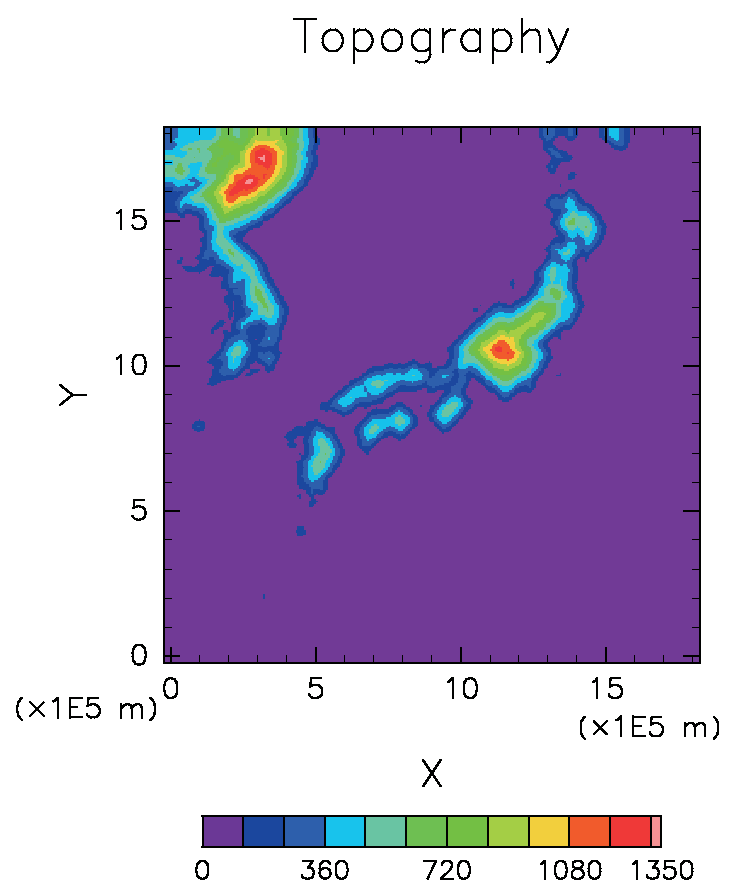
\includegraphics[width=0.5\hsize]{./figure/real_domain.eps}\\
  \caption{計算領域.カラーシェードは地形の標高を示す.}
  \label{fig:tutrial_real_domain}
\end{center}
\end{figure}


